%-----------------------------------------------------------------------------%
% Set metadata for use with pdfx
%\begingroup\newif\ifmy
%\IfFileExists{\jobname.xmpdata}{}{\mytrue}
%\ifmy
%\begin{filecontents*}{\jobname.xmpdata}
%\Title{Data Science Notes}
%\Author{Matthew Epland, Ph.D.}
%\Keywords{Data Science\sep Machine Learning\sep Statistics}
%\Copyright{CC-BY-4.0}
%\end{filecontents*}
%\fi\endgroup

% \Subject{TODO}

%-----------------------------------------------------------------------------%
% Set documentclass
\documentclass[nogradschool,singlespace,nobind]{dukedissertation_modified}

%-----------------------------------------------------------------------------%
% usepackages
\usepackage{amsmath,amssymb,bbm,bm} % https://ctan.org/pkg/bm
\usepackage{mathtools}
\usepackage{graphicx}
\usepackage{xcolor}
\usepackage{textcomp} % needed to fix \mico \textmu from siunitx to work with microtype: https://tex.stackexchange.com/questions/74670/microtype-siunitx-and-micro-mysterious-warnings
\usepackage[protrusion=true,expansion=true]{microtype} % make text flow nicely... might screw up duke dissertation template
\usepackage{verbatim} % verbatim text and comment environment
\usepackage{lmodern} % allowing font sizes at arbitrary sizes
\usepackage{notoccite} % fixes citation numbering in captions with respect to lof & lot, see https://ctan.org/pkg/notoccite
\usepackage[nocompress]{cite} % orders references numerically within one \cite{}, see https://tex.stackexchange.com/questions/69230/numbered-ordering-of-multiple-citations Also changes spacing after comma
\usepackage{fnpct} % make multiple footnotes at one point look nice, https://tex.stackexchange.com/questions/28465/multiple-footnotes-at-one-point
\usepackage[separate-uncertainty,multi-part-units=single,free-standing-units,product-units=repeat,use-xspace,binary-units]{siunitx} % units package, see https://www.ctan.org/pkg/siunitx
\sisetup{range-phrase={\text{--}},range-units=single}
\usepackage{physics}
\usepackage{booktabs,array,multirow,diagbox}
\renewcommand{\arraystretch}{1.5} % gives extra height to tabular rows for super/subscripts
%\usepackage{longtable}
\usepackage{enumitem}
\usepackage{lscape} % landscape https://ctan.org/pkg/lscape
\usepackage{moresize}
\usepackage{listings}
\usepackage[T1]{fontenc}

\usepackage[top=1in, bottom=1.25in, left=1.25in, right=1.25in]{geometry}
\usepackage{fancyhdr}
\pagestyle{plain}

% use subcaption to get split figures, but the caption dependency doesn't know about the dukedissertation document class - turn off the warning with silence
% load caption explicitly first to set it's options, subcaption says it passes them through but it doesn't seem to work
% https://tex.stackexchange.com/questions/34579/is-there-really-something-wrong-with-using-the-caption-package-for-continuedflo
% https://en.wikibooks.org/wiki/LaTeX/Floats,_Figures_and_Captions#Subfloats
% https://ctan.org/pkg/caption
% https://ctan.org/pkg/subcaption
\usepackage{silence}
\WarningFilter{caption}{Unsupported document class}
\WarningFilter{hyperref}{The PDF version number could not be set}
\usepackage{setspace} % needed to specify, https://ctan.org/pkg/setspace
\usepackage[style=base,skip=2pt,font={stretch=1.3},width=\textwidth]{caption}
\usepackage[skip=1pt]{subcaption}
\newsavebox{\largestimage} % see https://tex.stackexchange.com/questions/239128/subcaption-vertical-alignment-of-two-images-of-different-vertical-size

% Don't let floats get before the subsection where they're included
% https://tex.stackexchange.com/questions/32598/force-latex-image-to-appear-in-the-section-in-which-its-declared
% https://tex.stackexchange.com/questions/279/how-do-i-ensure-that-figures-appear-in-the-section-theyre-associated-with/235312#235312
% Also doesn't let a float go into a following subsection, results in a ton of blank space - probably better left off
% \usepackage{placeins}
%\let\Oldsubsection\subsection
%\renewcommand{\subsection}{\FloatBarrier\Oldsubsection}

\usepackage{float} % to allow for H option. Works better than \FloatBarrier from placeins, though it is more manual
\floatstyle{plaintop}
\restylefloat{table}

% keep footnotes from splitting, can still happen sometimes (10000 forces)
% https://tex.stackexchange.com/questions/32208/footnote-runs-onto-second-page
\interfootnotelinepenalty=9999

% keep inline equations from splitting, can still happen sometimes (10000 forces)
% https://tex.stackexchange.com/a/14243
\relpenalty=9999
\binoppenalty=9999

%-----------------------------------------------------------------------------%
% Other possibly useful packages
% \usepackage{fancyvrb}
% \usepackage{ulem}
% \usepackage{overpic}
% \usepackage{cancel}
% \usepackage{amsfonts, amsthm}
% \usepackage{mathabx}

%-----------------------------------------------------------------------------%
% tweak listings
\definecolor{codegreen}{rgb}{0,0.6,0}
\definecolor{codegray}{rgb}{0.5,0.5,0.5}
\definecolor{codemauve}{rgb}{0.58,0,0.82}

\lstset{
  backgroundcolor=\color{white},     % choose the background color; you must add \usepackage{color} or \usepackage{xcolor}; should come as last argument
  % basicstyle=\ssmall,                % the size of the fonts that are used for the code
  breakatwhitespace=false,           % sets if automatic breaks should only happen at whitespace
  breaklines=true,                   % sets automatic line breaking
  captionpos=b,                      % sets the caption-position to bottom
  commentstyle=\color{codegreen},    % comment style
  % deletekeywords={...},            % if you want to delete keywords from the given language
  % escapeinside={\%*}{*)},          % if you want to add LaTeX within your code
  extendedchars=true,                % lets you use non-ASCII characters; for 8-bits encodings only, does not work with UTF-8
  firstnumber=1,                     % start line enumeration with line 1000
  frame=none,                        % adds a frame around the code
  keepspaces=true,                   % keeps spaces in text, useful for keeping indentation of code (possibly needs columns=flexible)
  keywordstyle=\color{blue},         % keyword style
  % language=Octave,                 % the language of the code
  % morekeywords={*,...},            % if you want to add more keywords to the set
  numbers=left,                      % where to put the line-numbers; possible values are (none, left, right)
  numbersep=5pt,                     % how far the line-numbers are from the code
  numberstyle=\tiny\color{codegray}, % the style that is used for the line-numbers
  rulecolor=\color{black},           % if not set, the frame-color may be changed on line-breaks within not-black text (e.g. comments (green here))
  showspaces=false,                  % show spaces everywhere adding particular underscores; it overrides 'showstringspaces'
  showstringspaces=false,            % underline spaces within strings only
  showtabs=false,                    % show tabs within strings adding particular underscores
  stepnumber=1,                      % the step between two line-numbers. If it's 1, each line will be numbered
  stringstyle=\color{codemauve},     % string literal style
  tabsize=2,                         % sets default tabsize to 2 spaces
}

%-----------------------------------------------------------------------------%
% Include abbreviations
\usepackage{xspace}
 % note that \xspace properly handles the abbreviation period spacing - producing a single regular space, not the end of a sentence spacing

% https://tex.stackexchange.com/questions/7032/good-way-to-make-textcircled-numbers
% \usepackage{tikz}
% \DeclareRobustCommand{\circled}[1]{\tikz[baseline=(char.base)]{\node[shape=circle,draw,inner sep=1pt] (char) {#1};}}

% general, https://tex.stackexchange.com/questions/2229/is-a-period-after-an-abbreviation-the-same-as-an-end-of-sentence-period/2230#2230
\newcommand*{\ie}{\textit{i.e.}\@\xspace}
\newcommand*{\eg}{\textit{e.g.}\@\xspace}
%\newcommand*{\etc}{\textit{etc.}\@\xspace}
\makeatletter
\newcommand\etc{\textit{etc}\@ifnextchar.{}{.\@\xspace}}
\makeatother

% \newcommand{\orderof}{\ensuremath{\mathcal{O}}} % use \order from physics package instead
\newcommand{\lagr}{\ensuremath{\mathcal{L}}\xspace}
\newcommand{\transpose}{\ensuremath{^{\text{T}}}\xspace}
\newcommand{\stcomp}[1]{\overline{#1}}
\newcommand{\identity}{\ensuremath{I}\xspace} % note \mathbb{1} did not work
% \newcommand{\dif}{\mathop{}\!\mathrm{d}} % I think dt looks just fine
% \newcommand{\dif}{d} % I think dt looks just fine
\newcommand*{\dif}{\ensuremath{d}} % from ATLAS def

\DeclareMathOperator*{\sign}{sgn}

\DeclareMathOperator*{\argmin}{arg\,min} % thin space, limits underneath in displays, https://tex.stackexchange.com/questions/5223/command-for-argmin-or-argmax
\DeclareMathOperator*{\argmax}{arg\,max}

\newcommand*{\cov}[2]{\ensuremath{\text{cov}\left(#1,#2\right)}\xspace}
\newcommand*{\variance}[1]{\ensuremath{\text{var}\left(#1\right)}\xspace}
\newcommand*{\bias}[1]{\ensuremath{\text{bias}\left(#1\right)}\xspace}

\newcommand*{\expvalE}[1]{\ensuremath{E\left(#1\right)}\xspace}

\newcommand*{\pvalue}{\ensuremath{p\text{-value}}\xspace}

\newcommand*{\insitu}{\text{\textit{in~situ}}\xspace}
\newcommand*{\Insitu}{\text{\textit{In~situ}}\xspace}
\newcommand*{\InSitu}{\text{\textit{In~Situ}}\xspace}

\newcommand*{\apriori}{\text{\textit{a~priori}}\xspace}
\newcommand*{\aposteriori}{\text{\textit{a~posteriori}}\xspace}

\newcommand*{\CLs}{\ensuremath{CL_{s}}\xspace}

\newcommand*{\yhatBDT}{\ensuremath{\hat{y}_{\text{BDT}}}\xspace}
\newcommand*{\yhat}{\ensuremath{\hat{y}}\xspace}

% Software packages
\newcommand*{\xgboost}{\textsc{XGBoost}\xspace}
\newcommand*{\uprootPackage}{\textsc{uproot}\xspace} % \uproot already exists
\newcommand*{\python}{\textsc{Python}\xspace}
\newcommand*{\R}{\textsc{R}\xspace}
\newcommand*{\sql}{\textsc{SQL}\xspace}
\newcommand*{\pandas}{\textsc{Pandas}\xspace}
\newcommand*{\pyspark}{\textsc{PySpark}\xspace}
\newcommand*{\numpy}{\textsc{NumPy}\xspace}
\newcommand*{\scipy}{\textsc{SciPy}\xspace}
\newcommand*{\sklearn}{\textsc{Scikit-Learn}\xspace}
\newcommand*{\skopt}{\textsc{Scikit-Optimize}\xspace}
\newcommand*{\networkx}{\textsc{NetworkX}\xspace}
\newcommand*{\ROOT}{\textsc{ROOT}\xspace}
\newcommand*{\TMVA}{\textsc{TMVA}\xspace}
\newcommand*{\HF}{\textsc{HistFitter}\xspace}
\newcommand*{\hfactory}{\textsc{HistFactory}\xspace}
\newcommand*{\roostats}{\textsc{RooStats}\xspace}
\newcommand*{\roofit}{\textsc{RooFit}\xspace}


%-----------------------------------------------------------------------------%
% Include tikz figures which can not be made standalone, only if they have internal references / citations. Also must be manually added to Makefile if they use feynmp

%-----------------------------------------------------------------------------%
% Theorem, Lemma, etc. environments
%\newtheorem{theorem}{Theorem}%[section]
%\newtheorem{lemma}[theorem]{Lemma}
%\newtheorem{proposition}[theorem]{Proposition}
%\newtheorem{corollary}[theorem]{Corollary}
%\newtheorem{result}[theorem]{Result}

%-----------------------------------------------------------------------------%
% PREAMBLE
%-----------------------------------------------------------------------------%
\author{Matthew Epland, Ph.D.}
\title{Data Science Notes}
\date{\today}
%-----------------------------------------------------------------------------%

%-----------------------------------------------------------------------------%
% HYPERREF
%-----------------------------------------------------------------------------%
\usepackage[hyperpageref]{backref} % pages

% need to load in this order to get proper pdfx a-1b format!!!
\PassOptionsToPackage{hyperfootnotes,pagebackref}{hyperref}

% comment out if using pdfx
\usepackage{hyperref}
\makeatletter\hypersetup{
    breaklinks, baseurl=http://, pdfborder=0 0 0, pdfpagemode=UseNone, pdfstartpage=1, bookmarksopen=false, bookmarksdepth=2, % to show sections and subsections
    pdfauthor      = {Matthew Epland, Ph.D.}, %
    pdftitle       = {Data Science Notes}, %
    pdfsubject     = {Data Science, Machine Learning, Statistics}, %
    pdfkeywords    = {Data Science, Machine Learning, Statistics}
}\makeatother

% \usepackage[a-2b]{pdfx} % Note pdfx does not work with travis CI due to latest ubuntu image being from 2016, thus containing this bug https://bugs.debian.org/cgi-bin/bugreport.cgi?bug=877167 fixed in oct 2017. Can use locally if desired

\hypersetup{plainpages=false, bookmarksnumbered,
            % draft, % for printing
            colorlinks, linkcolor=blue, citecolor=blue, urlcolor=blue, % for web
            % breaklinks=true,
           }

% adapted from https://tex.stackexchange.com/questions/183702/formatting-back-references-in-bibliography-bibtex
\renewcommand*{\backrefalt}[4]{%
%    \ifcase #1 Not cited.%
    \ifcase #1% Not cited.%
          \or Cited on page~#2.%
          \else Cited on pages #2.%
    \fi%
    }

%-----------------------------------------------------------------------------%
% use cref and not ref, have to load last
\usepackage[capitalise]{cleveref} % https://ctan.org/pkg/cleveref see section 7.1, if redefining need to make them caps
\crefname{figure}{Figure}{Figures}
\Crefname{figure}{Figure}{Figures}
\crefname{tabular}{Table}{Tables}
\Crefname{tabular}{Table}{Tables}
\crefname{section}{Section}{Sections}
\Crefname{section}{Section}{Sections}
\crefname{chapter}{Chapter}{Chapters}
\Crefname{chapter}{Chapter}{Chapters}
\crefname{appchap}{Appendix}{Appendices}
\Crefname{appchap}{Appendix}{Appendices}
\crefformat{equation}{(#2#1#3)}

\newcommand\preface{%
   \nmchapter{Preface}
}

\begin{document}

%-----------------------------------------------------------------------------%
% TITLE PAGE
%-----------------------------------------------------------------------------%
\maketitle

%-----------------------------------------------------------------------------%
% ABSTRACT -- included file should start with '\abstract'.
%-----------------------------------------------------------------------------%
% \include{{sections/abstract}}

%-----------------------------------------------------------------------------%
% FRONTMATTER
%-----------------------------------------------------------------------------%
\tableofcontents % Automatically generated
\backrefsetup{disable}
\abbreviations

\section*{Symbols}

\begin{symbollist}
  \item[$P\left(X \mid Y\right)$] (Conditional) Probability of $X$ Given $Y$
  \item[$\expval{X}$ or $\expvalE{X}$] Expectation Value of $X$
  \item[$\sigma_{X}^{2}$ or $\variance{X}$] Variance of $X$
  \item[$\sigma_{u,v}^{2}$ or $\cov{u}{v}$] Covariance of $u$ and $v$
  \item[$\bm{\beta}$] Model Parameters, $n \times 1$ Column Vector
  \item[$\mathbf{X}$] Input Features, $m \times n$ Matrix
  \item[$y$] Dependent Feature
  \item[$m$] Number of Data Points or Rows% TODO sometimes n
  \item[$n$] Number of Input Features or Columns
  \item[$\nu$] Number of Degrees of Freedom
  \item[$S\left(\bm{\beta}\right)$] Objective Function
  \item[$L\left(\bm{\beta}\right)$] Loss Function
  \item[$\Omega\left(\bm{\beta}\right)$] Regularization Function
  \item[$L$] Likelihood Function
  \item[$\yhat$] Estimated Dependent Feature or Classification Score, Prediction
  \item[$Z$] Significance
  \item[$S\left(t\right)$] Survival Function
  \item[$\lambda\left(t\right)$] Hazard Function
  % \item[\ZB] Significance, Incomplete Beta Function Approximation
  % \item[\CLs] Signal Confidence Level
\end{symbollist}

\clearpage
\section*{Abbreviations}
% TODo keep updated

\begin{symbollist}
  \item[$k$-NN] $k$-Nearest Neighbors
  \item[ABC] Approximate Bayesian Computation
  \item[ACF] Auto-Correlation Function
  \item[ADF] Augmented Dickey--Fuller Test for Stationarity
  \item[AIC] Akaike Information Criterion
  \item[ANCOVA] Analysis of Covariance
  \item[ANOVA] Analysis of Variance
  \item[AR] Autoregressive (Models)
  \item[AUC] Area Under Curve
  \item[BDT] Boosted Decision Tree
  \item[BIC] Bayesian Information Criterion
  \item[BLUE] Best Linear Unbiased Estimator
  \item[CART] Classification and Regression Tree
  \item[CDF] Cumulative Distribution Function
  \item[CLT] Central Limit Theorem
  \item[CNN] Convolutional Neural Network
  \item[DID] Difference in Differences
  \item[FWHM] Full Width at Half Maximum
  \item[GLM] Generalized Linear Model
  \item[GLS] Generalized Least Squares
  \item[GMM] Gaussian Mixture Model
  \item[GP] Gaussian Process
  \item[HR] Hazard Ratio
  \item[i.i.d.] Independent and Identically Distributed
  \item[IQR] Interquartile Range
  \item[LSTM] Long Short Term Memory
  \item[LVQ] Learning Vector Quantization
  \item[MA] Moving Average (Models)
  \item[MANOVA] Multivariate Analysis of Variance
  \item[MAP] Maximum \aposteriori (Estimation)
  \item[MAPE] Mean Absolute Percent Error
  \item[MI] Mutual Information
  \item[ML] Machine Learning
  \item[MLE] Maximum Likelihood Estimation (or Estimator)
  \item[MMSE] Minimum Mean Square Error (Estimator)
  \item[MSE] Mean Squared Error
  \item[NMI] Normalized Mutual Information
  \item[NN] Neural Network
  \item[OLS] Ordinary Least Squares
  \item[PACF] Partial Auto-Correlation Function
  \item[PCA] Principle Component Analysis
  \item[PCR] Principal Component Regression
  \item[PDF] Probability Density Function
  \item[PR] Prevalence Ratio
  \item[RDBMS] Relational Database Management System
  \item[RMSD] Root Mean Squared Deviation
  \item[RMSE] Root Mean Squared Error
  \item[RNN] Recurrent Neural Network
  \item[ROC] Receiver Operating Characteristic
  \item[SGD] Stochastic Gradient Descent
  \item[SMBO] Sequential Model-Based Optimization
  \item[SQL] Structured Query Language
  \item[SVD] Singular Value Decomposition
  \item[SVM] Support Vector Machine
  \item[TPE] Tree-Structured Parzen Estimator
  \item[VIF] Variance Inflation Factor
%  \item[] 
\end{symbollist}
%  \item[GAN] Generational Adversarial Network
} % List of Abbreviations. Start file with '\abbreviations'
\backrefsetup{enable}

%-----------------------------------------------------------------------------%
% PREFACE
%-----------------------------------------------------------------------------%
\preface

These notes were prepared while studying data science interviews and are somewhat incomplete and scattered.
They are intended for use as a quick reference rather than an introduction to the material.
If you find an error, please let the author know at \href{https://www.linkedin.com/in/matthew-epland/}{{\small\faLinkedinSquare}~matthew-epland}.
You may also be interested in \textit{The Elements of Statistical Learning} \cite{HastieTF09},
and Doug Davis' lecture notes on the analysis of uncertainties \cite{DougNotes}.
}

%==============================================================================
%-----------------------------------------------------------------------------%
%
% MAIN BODY
%
%
%-----------------------------------------------------------------------------%
\chapter{Statistics}
\label{chap:stats}

%%%%%%%%%%%%%%%%%%%%%%%%%%%%%%%%%%%%%%%%%%%%%%%%%%%%%%%%
\section{Bayes' Theorem}
\label{stats:Bayes}

Bayes' theorem follows from the probability of the intersection of two events $A$ and $B$:

\begin{equation}\label{eq:stats:intersection}
P\left(A \cap B\right) = P\left(A \mid B\right) P\left(B\right) = P\left(B \mid A\right) P\left(A\right).
\end{equation}

\noindent Dividing by $P\left(B\right)$ we have:

\begin{equation}\label{eq:stats:Bayes}
\begin{split}
P\left(A \mid B\right) &= \frac{P\left(B \mid A\right) P\left(A\right)}{P\left(B\right)}\,, \\
&= \frac{P\left(B \mid A_{i}\right) P\left(A_{i}\right)}{\sum_{j} P\left(B \mid A_{j}\right)P\left(A_{j}\right)}\,, \\
\text{Posterior} &= \frac{\text{Likelihood} \times \text{Prior}}{\text{Normalization}}\,.
\end{split}
\end{equation}

Example: Testing for disease with a \SI{2}{\percent} incidence rate in the wider population.
The test has a \SI{99}{\percent} true positive rate and a \SI{15}{\percent} false positive rate.
What is the probability an individual has the disease if their test is positive?

\begin{equation}\label{eq:stats:BayesEx}
\begin{split}
P\left(\text{Infected} \mid +\right) &= \frac{P\left(+ \mid \text{Infected}\right) P\left(\text{Infected}\right)}{P\left(+\right)}\,, \\
 &= \frac{P\left(+ \mid \text{Infected}\right) P\left(\text{Infected}\right)}{
P\left(+ \mid \text{Infected}\right)P\left(\text{Infected}\right) + P\left(+ \mid \text{Healthy}\right)P\left(\text{Healthy}\right)}\,, \\
&= \frac{\num{0.99} \times \num{0.02}}{\num{0.99} \times \num{0.02} + \num{0.15} \times \left(1-\num{0.02}\right)}\,, \\
&\approx \num{0.57}\,.
\end{split}
\end{equation}

\noindent And if we run a second, independent, test which also comes back positive?

\begin{equation}\label{eq:stats:BayesEx2}
\begin{split}
P\left(\text{Infected} \mid ++\right) &= \frac{P\left(++ \mid \text{Infected}\right) P\left(\text{Infected}\right)}{P\left(++\right)}\,, \\
&= \frac{\num{0.99}^{2} \times \num{0.02}}{\num{0.99}^{2} \times \num{0.02} + \num{0.15}^{2} \times \left(1-\num{0.02}\right)}\,, \\
&\approx \num{0.90}\,.
\end{split}
\end{equation}

%%%%%%%%%%%%%%%%%%%%%%%%%%%%%%%%%%%%%%%%%%%%%%%%%%%%%%%%
% \section{Gaussian Distribution}
% \label{stats:gaus}
% TODO might not need

%%%%%%%%%%%%%%%%%%%%%%%%%%%%%%%%%%%%%%%%%%%%%%%%%%%%%%%%
% \section{Binomial Distribution}
% \label{stats:binomial}
% TODO

%%%%%%%%%%%%%%%%%%%%%%%%%%%%%%%%%%%%%%%%%%%%%%%%%%%%%%%%
% \section{Poisson Distribution}
% \label{stats:poisson}
% TODO

% \subsection{Bernoulli Distribution}
% \label{stats:poisson:bernoulli}
% TODO

%%%%%%%%%%%%%%%%%%%%%%%%%%%%%%%%%%%%%%%%%%%%%%%%%%%%%%%%
% \section{Maximum Likelihood Estimation (MLE)}
% \label{stats:MLE}
% TODO

%%%%%%%%%%%%%%%%%%%%%%%%%%%%%%%%%%%%%%%%%%%%%%%%%%%%%%%%
% \section{Principle Component Analysis (PCA)}
% \label{stats:PCA}
% TODO

%%%%%%%%%%%%%%%%%%%%%%%%%%%%%%%%%%%%%%%%%%%%%%%%%%%%%%%%
% \section{Analysis of Variance (ANOVA)}
% \label{stats:ANOVA}
% TODO

}
%%%%%%%%%%%%%%%%%%%%%%%%%%%%%%%%%%%%%%%%%%%%%%%%%%%%%%%%
%%%%%%%%%%%%%%%%%%%%%%%%%%%%%%%%%%%%%%%%%%%%%%%%%%%%%%%%
\chapter{Regression}
\label{chap:regression}

%%%%%%%%%%%%%%%%%%%%%%%%%%%%%%%%%%%%%%%%%%%%%%%%%%%%%%%%
%%%%%%%%%%%%%%%%%%%%%%%%%%%%%%%%%%%%%%%%%%%%%%%%%%%%%%%%
\section{Linear Regression}
\label{regression:linear}

Linear regression fits the best hyperplane, or line in 1D,
to a collection of $m$ points $\mathbf{x}_{i}, y_{i}$,
typically via the method of least squares.
If $\mathbf{x}$ has $n$ features we can represent the
linear relationship between $\mathbf{x}$ and $y$ as:

\begin{equation}\label{eq:linear:onepoint}
y_{i} = \beta_{0} + \sum_{j=1}^{n}\, \beta_{j} x_{ij} + \epsilon_{i}\,,
\end{equation}

\noindent where $\beta_{j}$ are the parameters of the regression
and $\epsilon$ represent random errors.
Transitioning to matrix notation\footnote{Note
that \textit{linear} regression refers to the linearity in the model parameters
$\bm{\beta}$, not $\mathbf{X}$.
The components of $\mathbf{X}_{i}$ can be, and often are,
non-linear functions of other input features.}, this is simply:

\begin{equation}\label{eq:linear:matrix}
\mathbf{y} = \mathbf{X} \bm{\beta} + \bm{\epsilon}\,,
\end{equation}

\noindent where we have set $X_{i0} =1$.

The ordinary least squares (OLS) estimate of the parameters $\hat{\bm{\beta}}$
can be found by minimizing the squares of the residuals,
\ie the objective function $S\left(\bm{\beta}\right)$:

\begin{subequations} \label{eq:linear:ols}
\begin{align}
\hat{\bm{\beta}} &= \argmin_{\bm{\beta}} S\left(\bm{\beta}\right)\,, \label{eq:linear:argmin} \\
S\left(\bm{\beta}\right) &= \sum_{i=1}^{m} \, \abs{y_{i} - \sum_{j=0}^{n} \, \beta_{j} x_{ij}}^{2} = \norm{\mathbf{y} - \mathbf{X} \bm{\beta}}^{2}\,. \label{eq:linear:S}
\end{align}
\end{subequations}

\noindent The optimal $\hat{\bm{\beta}}$ of \cref{eq:linear:ols} has a closed form solution:

\begin{equation}\label{eq:linear:betahat}
\hat{\bm{\beta}} = \left(\mathbf{X}\transpose\mathbf{X}\right)^{-1}\mathbf{X}\transpose \mathbf{y}\,,
\end{equation}

\noindent provided the following assumptions hold:

%%%%%%%%%%%%%%%%%%%%%%%%%%%%%%%%%%%%%%%%%%%%%%%%%%%%%%%%
\subsection{Assumptions}
\label{regression:linear:assumptions}

\begin{enumerate}[noitemsep]
\item The underlying relationship between $\mathbf{x}$ and $y$ is linear, and there are no major outliers.\label{item:regression:linear:linear}
\item The columns of $\mathbf{X}$, \ie features, are linearly independent, \ie $\mathrm{rank}\left(\mathbf{X}\right) = n$ (no multicollinearity).\label{item:regression:linear:multicollinearity}
\item The errors $\epsilon$ have conditional mean 0, $E\left(\epsilon \mid \mathbf{X}\right) = 0$ (exogeneity). The errors thus:\label{item:regression:linear:exogeneity}
\begin{enumerate}[noitemsep]
\item Have a mean of zero, $E\left(\epsilon\right) = 0$.
\item Are not correlated with the input features, $E\left(\mathbf{X}\transpose\epsilon\right) = 0$.
\end{enumerate}
\item The errors are spherical, $\mathrm{var}\left(\epsilon \mid \mathbf{X}\right) = \sigma^{2} \identity$. Thus:\label{item:regression:linear:spherical}
\begin{enumerate}[noitemsep]
\item Each observation $\mathbf{x}_{i}$ has the same constant variance $\sigma^{2}$ (homoscedasticity).
\item The errors are uncorrelated between observations, $E\left(\epsilon_{i}\epsilon_{j \neq i} \mid \mathbf{X}\right) = 0$ (no autocorrelation).
\end{enumerate}
\item The errors are normally distributed (multivariate normality)\footnote{This is not strictly required, but if true the OLS is the MLE and hypothesis testing works.}.\label{item:regression:linear:normality}
\end{enumerate}

If these assumptions are violated the following issues arise,
namely the model may be biased and or have a large or invalid estimated variance\footnote{A good reference may be found \href{http://people.duke.edu/~rnau/testing.htm}{here}.}:

\begin{itemize}[noitemsep]
\item[\ref{item:regression:linear:linear}.] If you are fitting nonlinear data the predictions will have large errors,
particularly when extrapolated beyond the range of the fitted data.
This will show up as systematic errors in the residuals plot,
or may be obvious when comparing observed vs predicted values.
Possible fixes include applying a nonlinear transformation to some of the features to linearize the data, \eg take the log,
adding more combinations of features, \eg higher polynomial terms,
or finding new independent features which may explain the nonlinearity.

\item[\ref{item:regression:linear:multicollinearity}.] If some of the features are not linearly independent (multicollinearity),
they can be biasing the model and should be removed in turn until linear independence is restored.
Multicollinearity can be spotted in the input feature correlation matrix,
or if the residuals correlate to any of the features.

\item[\ref{item:regression:linear:exogeneity}. \& \ref{item:regression:linear:spherical}.] If something is wrong with the errors
such that they correlate to the input features or across observations\footnote{Thus the residuals correlate with row number, \ie autocorrelation.},
have a non-zero mean, or have a changing variance,
the reported confidence intervals on the model parameters may be over or underestimated.

\item[\ref{item:regression:linear:normality}.] If the errors are not normally distributed the confidence intervals are again suspect.
This can be diagnosed by comparing the errors to the normal distribution with a normal probability plot, or normal quantile plot,
or through a statistical method like the Anderson-Darling and Kolmogorov-Smirnov tests.
Note that violating normality in the errors is not as much of an issue compared to the other assumptions
since the fit will still give usable coefficients provided the assumed form of the model is correct.
Problems of this kind can arise from nonlinear data or influential outliers.
If the errors really are non-normal, a generalized linear model (GLM) could be employed to model them correctly.
\end{itemize}

%%%%%%%%%%%%%%%%%%%%%%%%%%%%%%%%%%%%%%%%%%%%%%%%%%%%%%%%
\subsection{Goodness of Fit}
\label{regression:linear:goodness_of_fit}

% TODO R2, reduced chi square values, F-test, t-test

% TODO Ridge regression
% TODO Lasso regression

%%%%%%%%%%%%%%%%%%%%%%%%%%%%%%%%%%%%%%%%%%%%%%%%%%%%%%%%
%%%%%%%%%%%%%%%%%%%%%%%%%%%%%%%%%%%%%%%%%%%%%%%%%%%%%%%%
\section{Logistic Regression}
\label{regression:logistic}

Logistic regression is a simple method to create a classifier,
typically on two classes $y = 0,1$, though multinomial extensions exist.
Its name comes from the use of the logit, or log-odds, function

\begin{equation}\label{eq:logistic:logic}
l = \text{logit}\left(p\right) = \log\left(\frac{p}{1-p}\right)
\end{equation}

\noindent on the probability $p$ of class $1$.
$l$ is estimated linearly from $n$ input features $x_{j}$ with $n+1$ parameters $\beta_{j}$ as:

\begin{equation}\label{eq:logistic:logicBeta}
l = \beta_{0} + \sum_{j=1}^{n} \, \beta_{j}\,x_{j}\,.
\end{equation}

\noindent The probability $p$ is then

\begin{equation}\label{eq:logistic:p}
p = \frac{e^l}{e^l + 1} = \frac{1}{1+e^{-l}} = \text{logit}^{-1}\left(l\right)
\end{equation}

\noindent which can be turned into a predicted class through the choice of a suitable decision threshold.

The model parameters $\bm{\beta}$ are chosen by maximizing
the log of the likelihood $L$ \cref{eq:logistic:L} over $m$ known example points $\mathbf{x}_{i}, y_{i}$.
Note that $P\left(y \mid x\right)$ \cref{eq:logistic:Pr} is simply the Bernoulli distribution.
In practice the log-likelihood $\log\left(L\right)$ is maximized via gradient descent.
An example of logistic regression can be found in \cref{fig:logistic_regression_ex}.

\begin{subequations} \label{eq:logistic:L_Pr}
\begin{align}
L\left(\bm{\beta} \mid \mathbf{x}\right) &= \prod_{i=1}^{m} \, P\left(y_{i} \mid \mathbf{x}_{i};\,\bm{\beta}\right) \label{eq:logistic:L} \\
P\left(y \mid \mathbf{x}\right) &= p^y\left(1-p\right)^{1-y}, \quad y \in \{0, 1\} \label{eq:logistic:Pr}
\end{align}
\end{subequations}

\begin{figure}
\centering
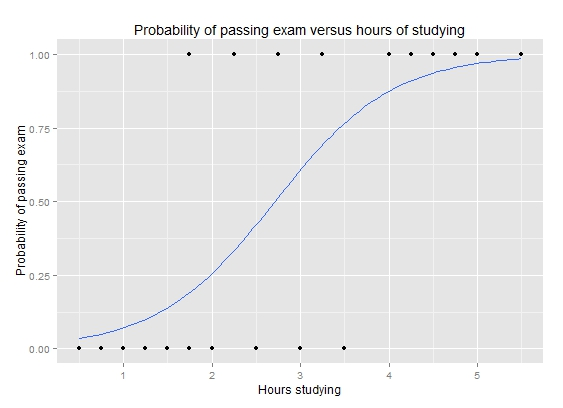
\includegraphics[width=0.8\textwidth]{figures/regression/Exam_pass_logistic_curve.jpeg}
\caption{
Example logistic regression curve on one input feature, by \href{https://en.wikipedia.org/wiki/File:Exam_pass_logistic_curve.jpeg}{Michaelg2015}.
}
\label{fig:logistic_regression_ex}
\end{figure}

Some assumptions of the logistic regression approach are:
\begin{enumerate}[noitemsep]
\item $y$ is either present or absent (dichotomous).
\item There are minimal correlations between the $x_{j}$ features (no multicollinearity).
\item There are no major outliers in the data.
\end{enumerate}

% TODO pseudo R2, Wald statistic

%%%%%%%%%%%%%%%%%%%%%%%%%%%%%%%%%%%%%%%%%%%%%%%%%%%%%%%%
%%%%%%%%%%%%%%%%%%%%%%%%%%%%%%%%%%%%%%%%%%%%%%%%%%%%%%%%
\section{Gaussian Process Regression}
\label{Regression:kriging}
% TODO also known as kriging

}
%%%%%%%%%%%%%%%%%%%%%%%%%%%%%%%%%%%%%%%%%%%%%%%%%%%%%%%%
%%%%%%%%%%%%%%%%%%%%%%%%%%%%%%%%%%%%%%%%%%%%%%%%%%%%%%%%
%%%%%%%%%%%%%%%%%%%%%%%%%%%%%%%%%%%%%%%%%%%%%%%%%%%%%%%%
% \chapter{Machine Learning}
% \label{ml}

%%%%%%%%%%%%%%%%%%%%%%%%%%%%%%%%%%%%%%%%%%%%%%%%%%%%%%%%
%%%%%%%%%%%%%%%%%%%%%%%%%%%%%%%%%%%%%%%%%%%%%%%%%%%%%%%%
%%%%%%%%%%%%%%%%%%%%%%%%%%%%%%%%%%%%%%%%%%%%%%%%%%%%%%%%
\chapter{General Machine Learning Concepts}
\label{ml:general}

%%%%%%%%%%%%%%%%%%%%%%%%%%%%%%%%%%%%%%%%%%%%%%%%%%%%%%%%
%%%%%%%%%%%%%%%%%%%%%%%%%%%%%%%%%%%%%%%%%%%%%%%%%%%%%%%%
\section{Evaluating Performance}
\label{ml:general:eval}

%%%%%%%%%%%%%%%%%%%%%%%%%%%%%%%%%%%%%%%%%%%%%%%%%%%%%%%%
\subsection{Confusion Matrix}
\label{ml:general:eval:cm}

The confusion matrix is a simple table of the number of actual, or truth, class instances
versus the number of a model's predicted class instances.
A two class example is provided in \cref{table:CM}.
Multi-class confusion matrices are straight forward extensions,
with correctly classified instances appearing along the diagonal.

\begin{table}[H]
  \centering
  \begin{tabular}{c | c | c | c |}
  \multicolumn{2}{c}{} & \multicolumn{2}{c}{\textbf{Actual}} \\ \cline{3-4}
  \multicolumn{1}{c}{} & & Positive & Negative \\ \cline{2-4}
  \multirow{4}{*}{\rotatebox{90}{\textbf{Predicted}}} & \multirow{2}{*}{Positive} & \multirow{2}{*}{TP} & FP \\[-8pt]
   & & & (Type I) \\ \cline{2-4}
   & \multirow{2}{*}{Negative} & FN & \multirow{2}{*}{TN} \\[-8pt]
   & & (Type II) & \\ \cline{2-4}
  \end{tabular}
  \caption{Two class confusion matrix.}
  \label{table:CM}
\end{table}

%%%%%%%%%%%%%%%%%%%%%%%%%%%%%%%%%%%%%%%%%%%%%%%%%%%%%%%%
\subsection{TPR \& TNR -- Sensitivity \& Specificity}
\label{ml:general:eval:TPR_TNR}

The true positive rate (TPR) and true negative rate (TNR) are
relatively straight forward to compute and understand, along with their complements,
the false negative rate (FNR), \ie miss rate, and false positive rate (FPR), \ie fall-out.
Here the denominators are the number of true class members.

\begin{enumerate}[noitemsep]
\item True positive rate (TPR), \ie sensitivity, recall, hit rate:
\begin{equation} \label{eq:TPR}
\text{TPR} = \frac{\text{TP}}{\text{P}} = \frac{\text{TP}}{\text{TP}+\text{FN}} = 1 - \text{FNR} = P\left(\hat{+} \mid + \right)
\end{equation}

\item True negative rate (TNR), \ie specificity, selectivity:
\begin{equation} \label{eq:TNR}
\text{TNR} = \frac{\text{TN}}{\text{N}} = \frac{\text{TN}}{\text{TN}+\text{FP}} = 1 - \text{FPR} = P\left(\hat{-} \mid - \right)
\end{equation}
\end{enumerate}

%%%%%%%%%%%%%%%%%%%%%%%%%%%%%%%%%%%%%%%%%%%%%%%%%%%%%%%%
\subsection{PPV (Precision) \& NPV}
\label{ml:general:eval:PPV_NPV}

The positive predictive value (PPV), more commonly known as precision, and negative predictive value (NPV)
are related metrics, but with predicted class members in the denominators.
Their complements are the false discovery rate (FDR) and false omission rate (FOR).
It is helpful to look at these metrics graphically, as in \cref{fig:graphical_CM_quantities}.

\begin{enumerate}[noitemsep]
\item Positive predictive value (PPV), \ie precision:
\begin{equation} \label{eq:PPV}
\text{PPV} = \frac{\text{TP}}{\hat{\text{P}}} = \frac{\text{TP}}{\text{TP}+\text{FP}} = 1 - \text{FDR} = P\left(+ \mid \hat{+} \right)
\end{equation}

\item Negative predictive value (NPV):
\begin{equation} \label{eq:NPV}
\text{NPV} = \frac{\text{TN}}{\hat{\text{N}}} = \frac{\text{TN}}{\text{TN}+\text{FN}} = 1 - \text{FOR} = P\left(- \mid \hat{-} \right)
\end{equation}
\end{enumerate}

\begin{figure}[H]
\centering
  \begin{subfigure}[c]{0.48\textwidth}\centering
  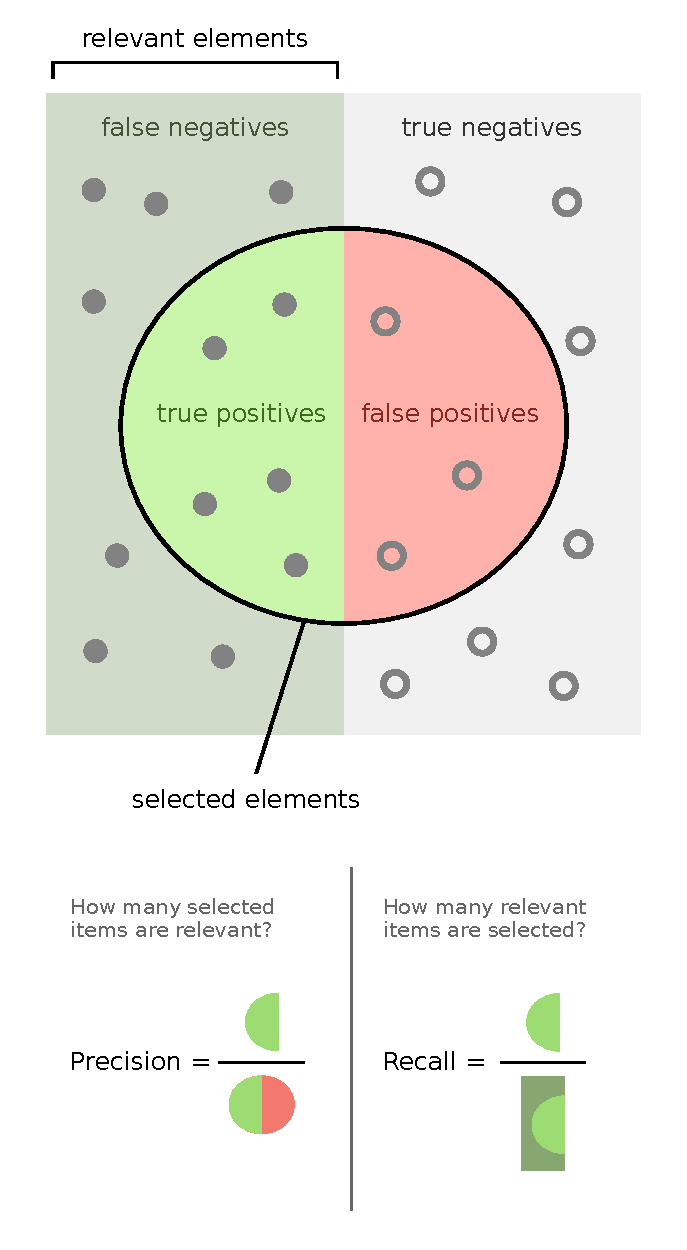
\includegraphics[width=\textwidth]{figures/ml/precision_recall.pdf}
  \caption{Precision \& Recall}
  \label{fig:graphical_CM_quantities:precision_recall}
  \end{subfigure}
  ~
  \begin{subfigure}[c]{0.48\textwidth}\centering
  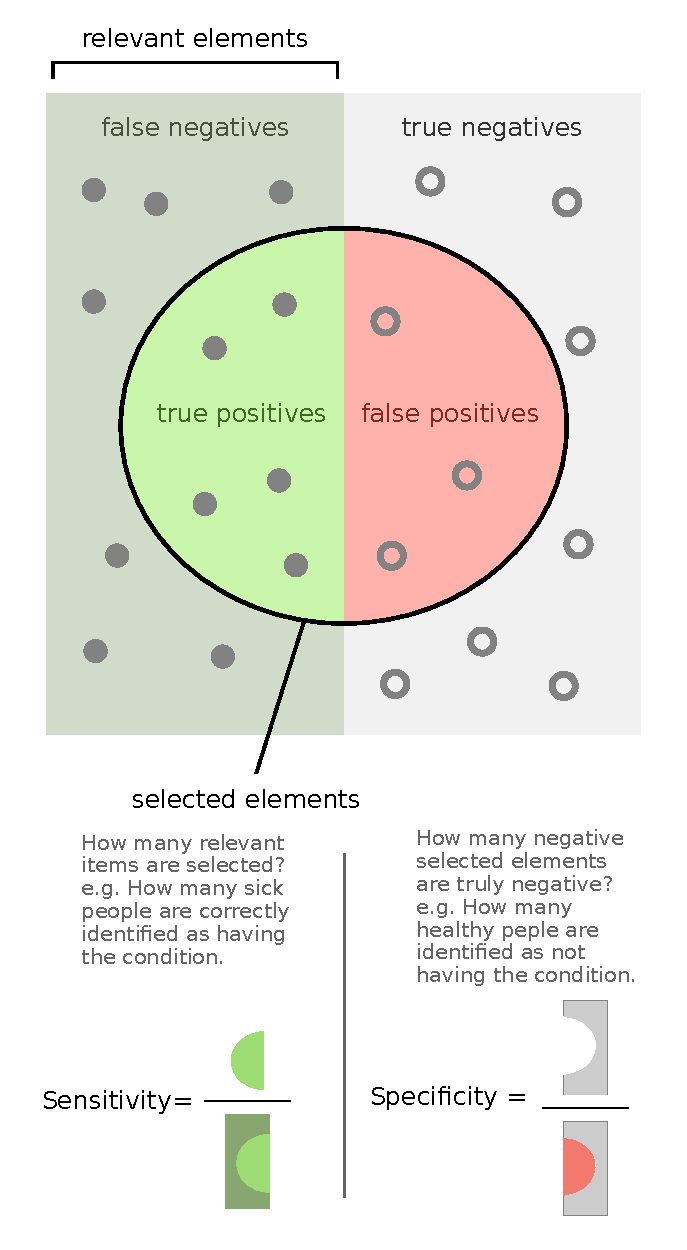
\includegraphics[width=\textwidth]{figures/ml/sensitivity_and_specificity.pdf}
  \caption{Sensitivity \& Specificity}
  \label{fig:graphical_CM_quantities:sensitivity_specificity}
  \end{subfigure}
\caption{
Graphical representation of
precision versus recall (sensitivity), by \href{https://commons.wikimedia.org/wiki/File:Precisionrecall.svg}{Walber},
and
sensitivity (recall) versus specificity, by \href{http://en.wikipedia.org/wiki/File:Sensitivity_and_specificity.svg}{FeanDoe}.
}
\label{fig:graphical_CM_quantities}
\end{figure}

%%%%%%%%%%%%%%%%%%%%%%%%%%%%%%%%%%%%%%%%%%%%%%%%%%%%%%%%
\subsection{Other Scores}
\label{ml:general:eval:other_scores}

The accuracy (ACC), the proportion of correct predictions, is a natural metric for measuring a classifiers performance.
Various F-scores, such as $F_{1}$ and $F_{\beta}$, combine precision and recall into one metric\footnote{Note that $F_{\beta}$ does not depend on TN at all, a potential shortcoming.}.
$F_{1}$ balances precision and recall equally, and is their harmonic mean,
while $F_{\beta}$ uses $\beta$ to assign different weights to each\footnote{$F_{2}$ weights recall over precision, $F_{0.5}$ weights precision over recall.}.

\begin{enumerate}[noitemsep]
\item Accuracy (ACC):
\begin{equation} \label{eq:ACC}
\text{ACC} = \frac{\text{TP}+\text{TN}}{\text{P}+\text{N}} = \frac{\text{TP}+\text{TN}}{\text{TP}+\text{TN}+\text{FP}+\text{FN}}
\end{equation}

\item $F_{1}$ ($F_{1}=1$ is best, $F_{1}=0$ is worst):
\begin{equation} \label{eq:F1}
F_{1} = \left(\frac{\text{precision}^{-1}+\text{recall}^{-1}}{2}\right)^{-1} = 2\,\,\frac{\text{precision} \times \text{recall}}{\text{precision} + \text{recall}}
\end{equation}

\item $F_{\beta}$ (Larger $\beta$ weights recall over precision):
\begin{equation} \label{eq:Fbeta}
F_{\beta} = \left(1+\beta^{2}\right) \frac{\text{precision} \times \text{recall}}{\beta^{2}\,\text{precision} + \text{recall}} =
\frac{\left(1+\beta^{2}\right) \text{TP}}{\left(1+\beta^{2}\right) \text{TP} + \beta^{2}\,\text{FN} + \text{FP}}
\end{equation}
\end{enumerate}

\clearpage% TODo hard coded
%%%%%%%%%%%%%%%%%%%%%%%%%%%%%%%%%%%%%%%%%%%%%%%%%%%%%%%%
%%%%%%%%%%%%%%%%%%%%%%%%%%%%%%%%%%%%%%%%%%%%%%%%%%%%%%%%
\section{Bias-Variance Tradeoff}
\label{ml:general:bias_variance_tradeoff}

\begin{enumerate}[noitemsep]
\item Bias: Errors due to a model not learning about relationships between features in the training data, \ie underfitting. Caused by invalid relationships present in the model.
\item Variance: Errors due to an overly complex model failing to generalize beyond the training data, \ie overfitting. Caused by sensitivity to small fluctuations in the training data.
\end{enumerate}

\begin{figure}[H]
  \centering
  \savebox{\largestimage}{
    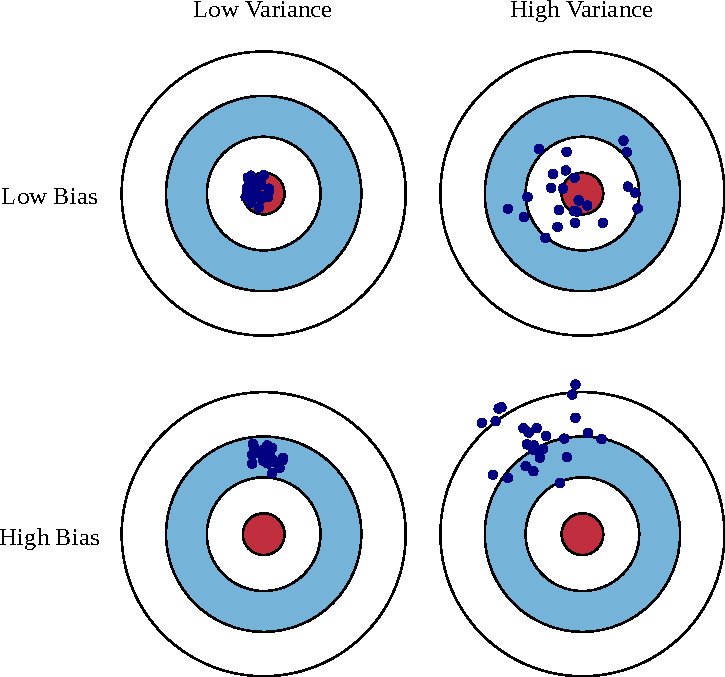
\includegraphics[width=0.47\textwidth]{figures/ml/bias_variance_tradeoff.pdf}
  }% Store largest image in a box

  \begin{subfigure}[b]{0.48\textwidth}\centering
    \usebox{\largestimage}
    \vspace{0.01cm}
  \caption{Direct Comparison}
  \label{fig:ml:bias_variance_tradeoff:direct}
  \end{subfigure}
  ~
  \begin{subfigure}[b]{\wd\largestimage}\centering
    \raisebox{\dimexpr.5\ht\largestimage-.5\height}{% Adjust vertical height of smaller image
      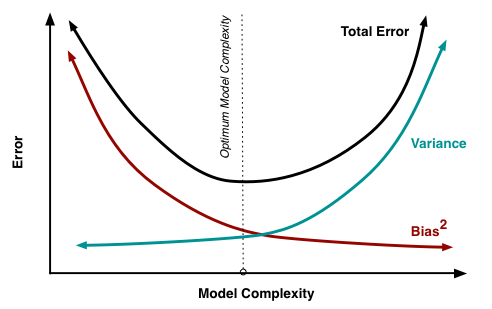
\includegraphics[width=\textwidth]{figures/ml/bias_variance_error_tradeoff.png}}
  \caption{Error Components (Test Set)}
  \label{fig:ml:bias_variance_tradeoff:error}
  \end{subfigure}
\caption{
Illustrations of the bias-variance tradeoff,
by \href{http://scott.fortmann-roe.com/docs/BiasVariance.html}{Scott Fortmann-Roe}.
\label{fig:ml:bias_variance_tradeoff}
}
\end{figure}

Every model makes a tradeoff between bias and variance,
which is roughly controlled by its level of complexity
as can be seen in \cref{fig:ml:bias_variance_tradeoff:error}.
\Cref{fig:additional:ml:general:early_stopping} shows this in practice,
as past a certain point of complexity the validation error grows
while the training error continues to decrease.

\subsubsection{Mean Square Error (MSE) Decomposition}
\label{ml:general:bias_variance_tradeoff:decop}

We can analytically decompose the mean square error (MSE) into explicit
bias, variance, and irreducable error components.
Let $y = f\left(\mathbf{x}\right) + \epsilon$ represent
the observed data, $y_{i}$, $\mathbf{x}_{i}$,
where $f\left(\mathbf{x}\right)$ is the true parent distribution\footnote{$\expval{f} = f$ is deterministic,
and acts as a constant as far as expectation values are concerned.} and
$\epsilon$ is random noise\footnote{This is the source of the irreducible error.
Since future data will still have $\epsilon$, the predictions can't be perfect
-- even when neglecting the model's own bias and variance.}\footnote{Later we'll need
$\sigma^{2} = \variance{\epsilon} = \expval{\epsilon^{2}} - \expval{\epsilon}^{2} = \expval{\epsilon^{2}}$.} having
$\expval{\epsilon} = 0$, $\variance{\epsilon} = \sigma^{2}$.
Representing the trained model\footnote{Note
that $\cov{\epsilon}{\hat{f}} = 0 \Rightarrow \expval{\epsilon \hat{f}} = \expval{\epsilon} \expval{\hat{f}}$.} as
$\hat{f}\left(\mathbf{x}\right)$, we expand the MSE:

\begin{subequations} \label{eq:bias_variance_tradeoff:decop}
\begin{align}
\text{MSE} &= \expval{\left(y-\hat{f}\right)^{2}} \\
&= \expval{\left(f + \epsilon - \hat{f} + \big[\expval{\hat{f}}-\expval{\hat{f}}\big]\right)^{2}}\,, \\
&= \expval{\left(\big[f - \expval{\hat{f}}\big] + \epsilon - \big[\hat{f} - \expval{\hat{f}}\big]\right)^{2}}\,, \\
&= \expval{\left(f-\expval{\hat{f}}\right)^{2}}
+\expval{\epsilon^{2}}
+\expval{\left(\hat{f}-\expval{\hat{f}}\right)^{2}}
+2\expval{\left(f-\expval{\hat{f}}\right)\epsilon} \\
&\hphantom{=}-2\expval{\epsilon\left(\hat{f}-\expval{\hat{f}}\right)}
-2\expval{\left(f-\expval{\hat{f}}\right)\left(\hat{f}-\expval{\hat{f}}\right)}\,, \\
&= \left(-1\right)^{2}\left(\expval{\hat{f}}-f\right)^{2} +\sigma^{2} + \variance{\hat{f}}
+2\left(f-\expval{\hat{f}}\right)\cancelto{0}{\expval{\epsilon}} \\
&\hphantom{=}-2\cancelto{0}{\expval{\epsilon}}\left(\expval{\hat{f}}-\expval{\hat{f}}\right)
-2\left(f-\expval{\hat{f}}\right)\cancelto{0}{\left(\expval{\hat{f}}-\expval{\hat{f}}\right)}\,, \\
&= \left(\bias{\hat{f}}\right)^{2} + \variance{\hat{f}} + \sigma^{2}\,.
\end{align}
\end{subequations}

\clearpage% TODo hard coded
%%%%%%%%%%%%%%%%%%%%%%%%%%%%%%%%%%%%%%%%%%%%%%%%%%%%%%%%
%%%%%%%%%%%%%%%%%%%%%%%%%%%%%%%%%%%%%%%%%%%%%%%%%%%%%%%%
\section{Regularization}
\label{ml:general:reg}

Regularization is a method for controlling the variance (overfitting)
of a model by putting constraints on the size of its parameters.
In terms of \cref{ml:general:bias_variance_tradeoff}, regularization forces the model's
bias to grow on the training set in order to lower the variance on future data.
The two main types of regularization are shown in \cref{eq:L1_L2}
and depend on different powers of the norm\footnote{In
the case of OLS linear regression the constant intercept term $\beta_{0}$ is not included in $\norm{\bm{\beta}}$.} of the model parameters $\bm{\beta}$.
In order to treat all features equally, normalization must be used before applying regularization.
A hyperparameter $\lambda$ is included to tune the amount of regularization applied in the objective function,
$S\left(\bm{\beta}\right) = L + \Omega$.
As $\lambda$ is increased, it decreases the size the model's coefficients, and thereby its variance (overfitting),
up to a point when the model is unable to adequately train on the available data and the bias (underfitting) begins to grow.

\begin{subequations} \label{eq:L1_L2}
\begin{align}
\Omega_{\text{L1}}\left(\bm{\beta}\right) &= \lambda \norm{\bm{\beta}}\hphantom{^{1}}
= \lambda \sum_{j=1}^{n} \, \abs{\beta_{j}}\,, \label{eq:L1} \\
\Omega_{\text{L2}}\left(\bm{\beta}\right) &= \lambda \norm{\bm{\beta}}^{2}
= \lambda \sum_{j=1}^{n} \,\, \beta_{j}^{2}\,. \label{eq:L2}
\end{align}
\end{subequations}

For a particular value of $\lambda$, the effect of L1 and L2 regularization\footnote{Here
$q$ is being used as the power of $\norm{\bm{\beta}}$. For L1 (L2), $q=1$ ($q=2$).} is
to constrain $\norm{\bm{\beta}}^{q} \leq t\left(\lambda\right)$ for some $t\left(\lambda\right)$.
As can be seen in \cref{fig:ml:l1l2} the L1 norm constrains $\bm{\beta}$ to lie within a hypercube,
while the L2 constraint is a hypersphere.

\begin{figure}[H]
  \centering
  \begin{subfigure}[b]{0.48\textwidth}\centering
      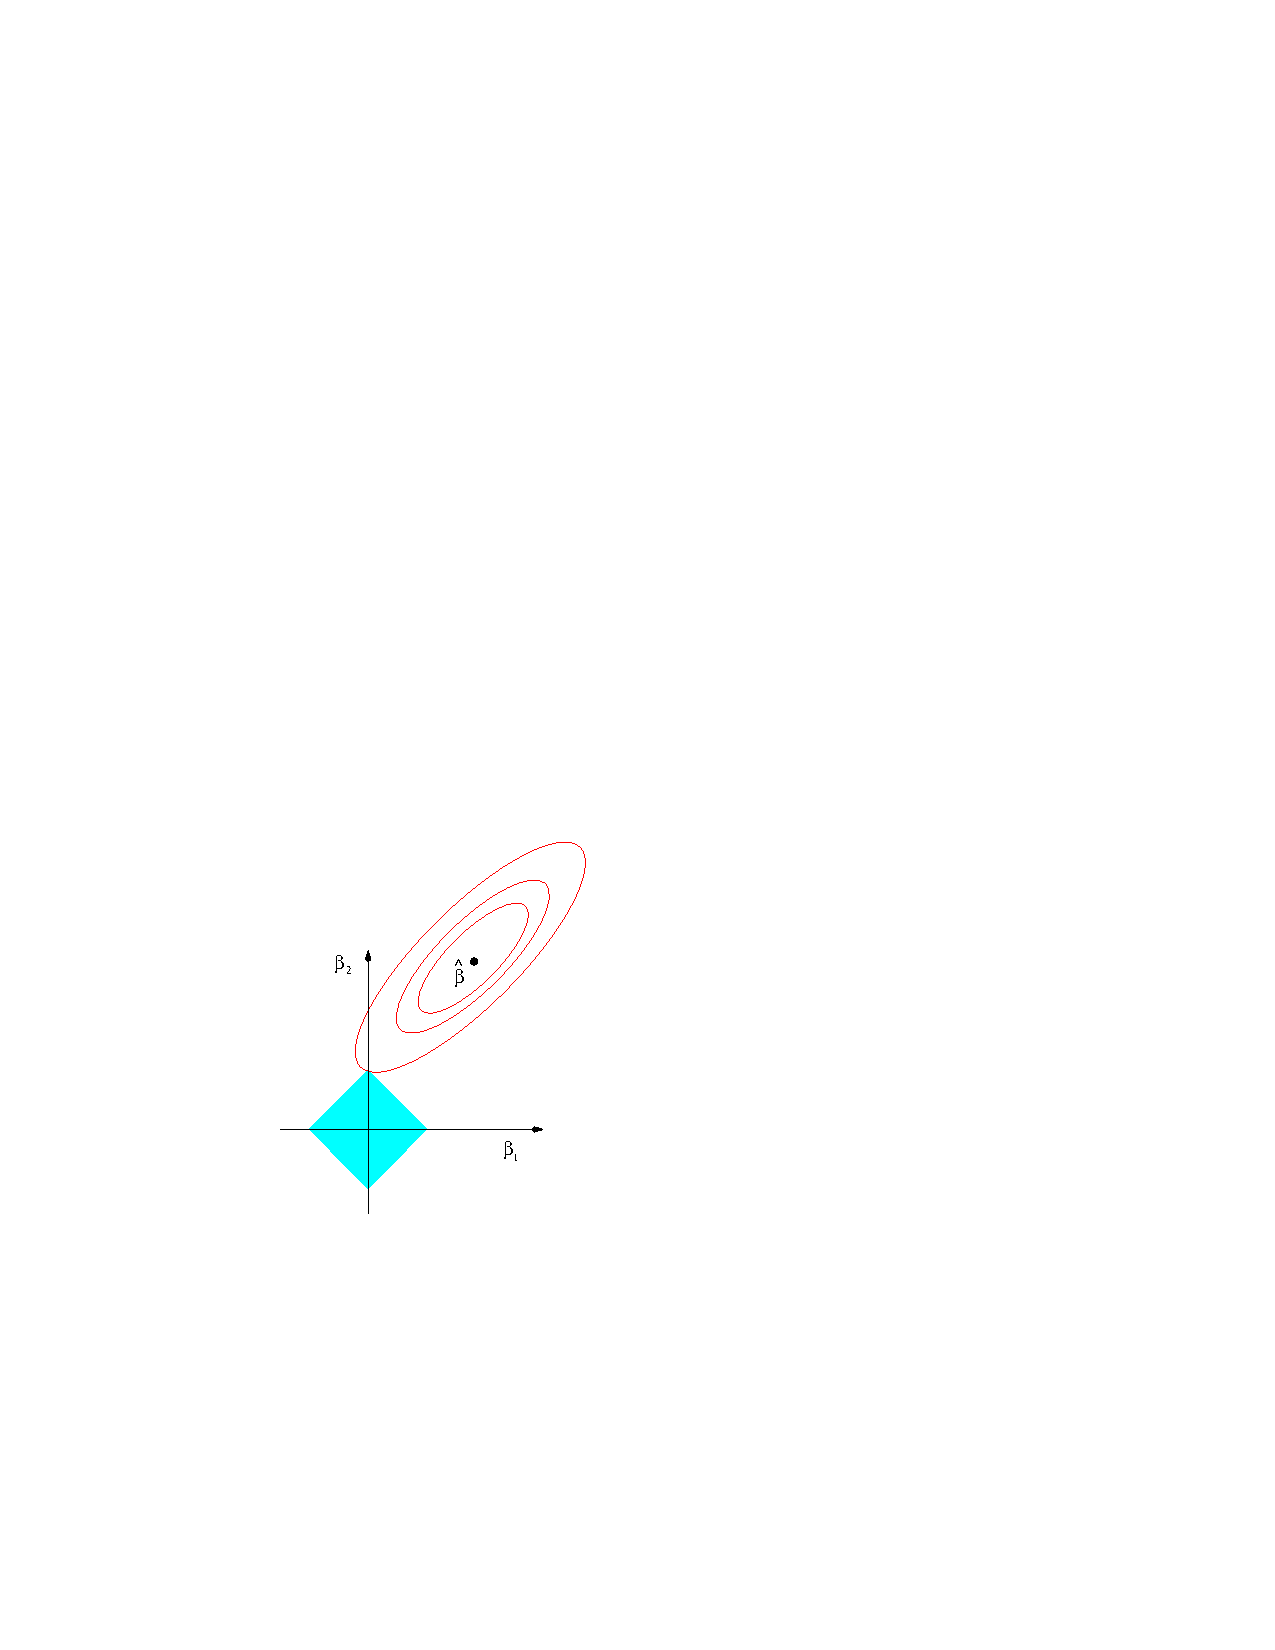
\includegraphics[width=\textwidth]{figures/ml/l1.pdf}
  \caption{L1}
  \label{fig:ml:l1l2:l1}
  \end{subfigure}
  ~
  \begin{subfigure}[b]{0.48\textwidth}\centering
      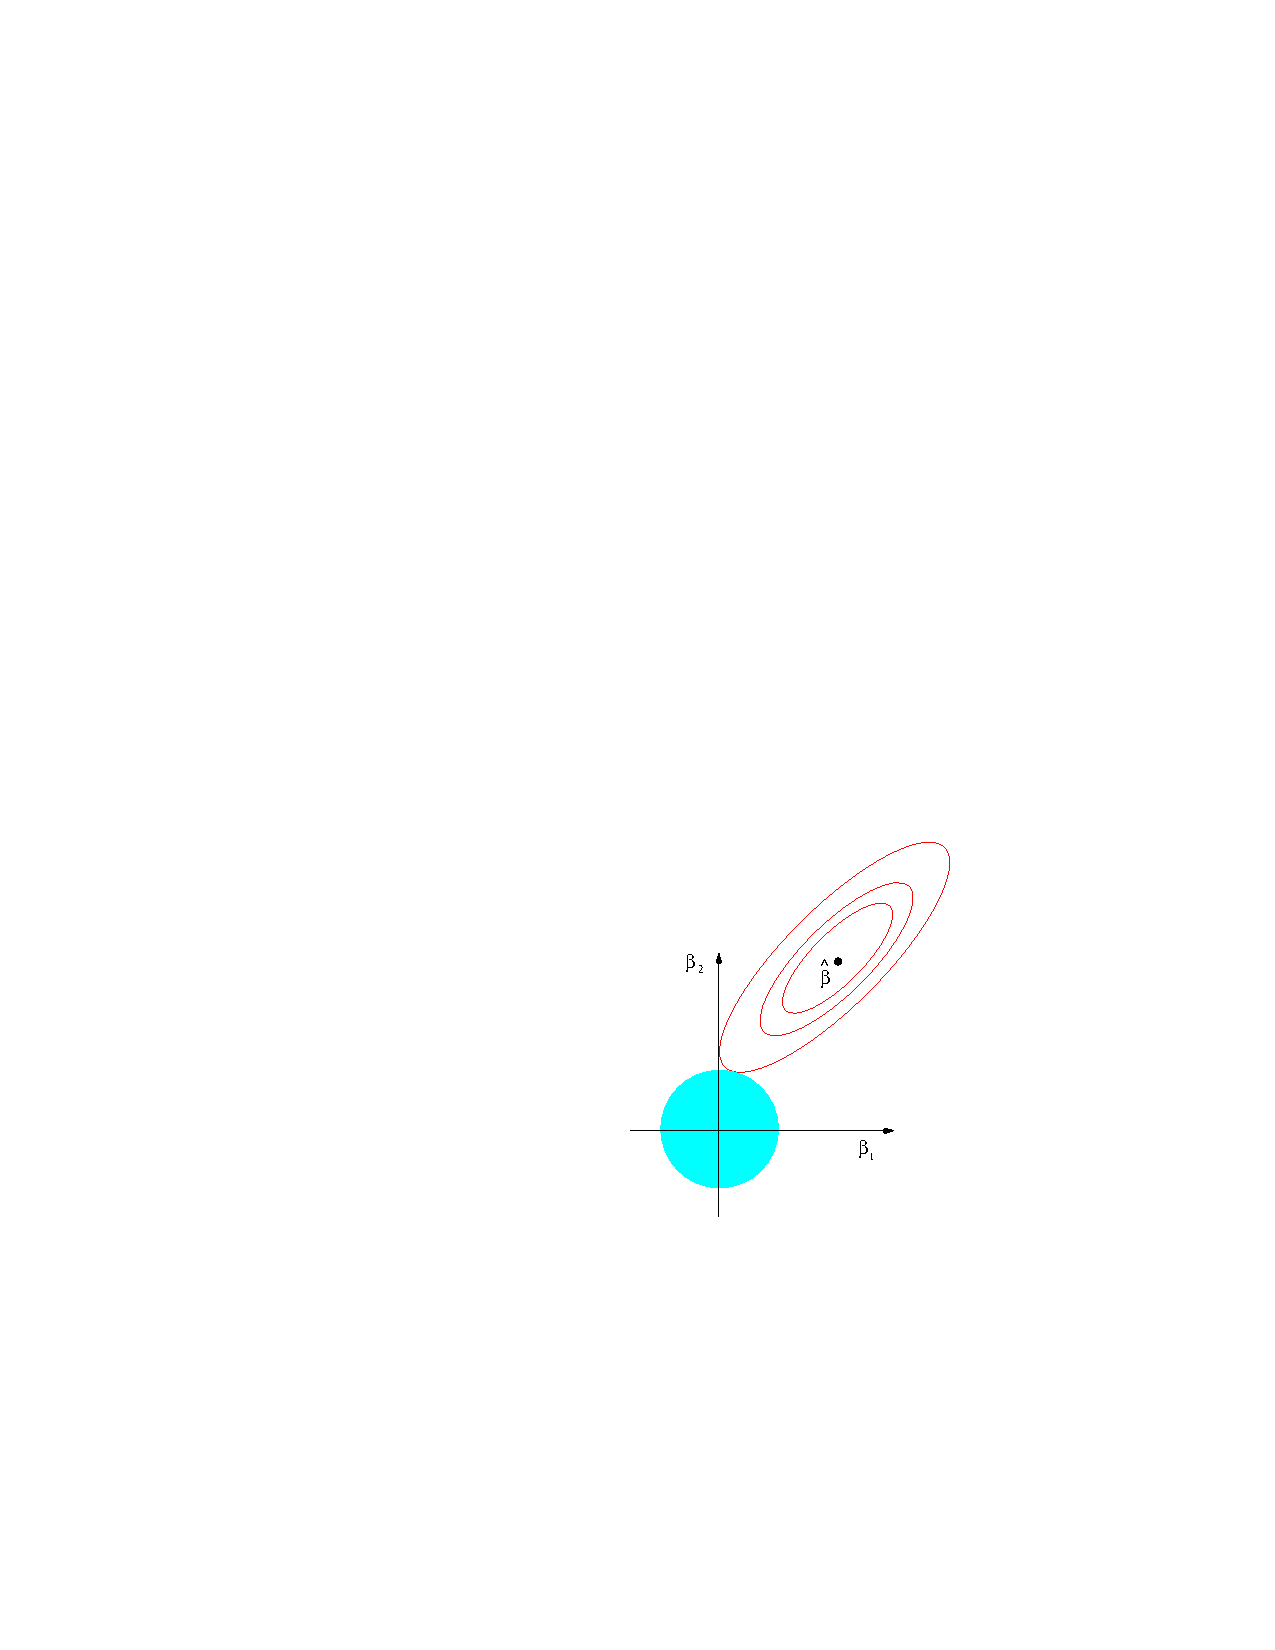
\includegraphics[width=\textwidth]{figures/ml/l2.pdf}
  \caption{L2}
  \label{fig:ml:l1l2:L2}
  \end{subfigure}
\caption{
A graphical representation of the L1 and L2 regularization constraints on $\bm{\beta}$ \cite{HastieTF09}.
The best value of $\bm{\beta}$ for optimizing the loss function $L$ is indicated as $\hat{\bm{\beta}}$.
For a given contour in $L$, L1 will tend to force $\bm{\beta}$ along one of the axes,
identically setting some $\beta_{i}$ coefficients to zero,
while L2 is rotationally symmetric and has no such tendencies.
\label{fig:ml:l1l2}
}
\end{figure}

%%%%%%%%%%%%%%%%%%%%%%%%%%%%%%%%%%%%%%%%%%%%%%%%%%%%%%%%
\subsection{L1 -- LASSO}
\label{ml:general:reg:L1}
L1, or LASSO\footnote{Least absolute shrinkage and selection operator.},
regularization uses the norm $\norm{\bm{\beta}}$ \cref{eq:L1}, or taxi cab distance.
As it's geometric constraints on $\bm{\beta}$ are hypercubes,
it tends to set some model parameters to 0, creating sparsity,
and thereby acts as a form of built-in feature selection.

%%%%%%%%%%%%%%%%%%%%%%%%%%%%%%%%%%%%%%%%%%%%%%%%%%%%%%%%
\subsection{L2 -- Ridge}
\label{ml:general:reg:L2}
L2, or ridge, regularization \cref{eq:L2} uses the square of the norm, or euclidean distance.
Models made with L2 regularization are somewhat less interpretable than those made with L1,
as L2 may make many parameters very small, but does not remove them entirely.
The parameters are still shrunk toward zero, and each other,
while highly correlated features are effectively averaged.
L2 is slightly faster to run than L1 computationally as, unlike L1, it
is not represented as a piecewise function and has a closed form expression.

%%%%%%%%%%%%%%%%%%%%%%%%%%%%%%%%%%%%%%%%%%%%%%%%%%%%%%%%
%%%%%%%%%%%%%%%%%%%%%%%%%%%%%%%%%%%%%%%%%%%%%%%%%%%%%%%%
\section{Gradient Descent}
\label{ml:general:grad_descent}
% TODO

%%%%%%%%%%%%%%%%%%%%%%%%%%%%%%%%%%%%%%%%%%%%%%%%%%%%%%%%
\subsection{Stochastic Gradient Descent (SGD)}
\label{ml:general:grad_descent:stochastic}
% TODO


%%%%%%%%%%%%%%%%%%%%%%%%%%%%%%%%%%%%%%%%%%%%%%%%%%%%%%%%
%%%%%%%%%%%%%%%%%%%%%%%%%%%%%%%%%%%%%%%%%%%%%%%%%%%%%%%%
%%%%%%%%%%%%%%%%%%%%%%%%%%%%%%%%%%%%%%%%%%%%%%%%%%%%%%%%
\chapter{Unsupervised Learning}
\label{ml:unsupervised}

%%%%%%%%%%%%%%%%%%%%%%%%%%%%%%%%%%%%%%%%%%%%%%%%%%%%%%%%
%%%%%%%%%%%%%%%%%%%%%%%%%%%%%%%%%%%%%%%%%%%%%%%%%%%%%%%%
\section{\texorpdfstring{$k$}{k}-Means}
\label{ml:unsupervised:kMean}
% TODO

%%%%%%%%%%%%%%%%%%%%%%%%%%%%%%%%%%%%%%%%%%%%%%%%%%%%%%%%
\subsection{Metrics}
\label{ml:unsupervised:kMean:metrics}
% TODO describe both cartesian and cosine similarity metrics


%%%%%%%%%%%%%%%%%%%%%%%%%%%%%%%%%%%%%%%%%%%%%%%%%%%%%%%%
%%%%%%%%%%%%%%%%%%%%%%%%%%%%%%%%%%%%%%%%%%%%%%%%%%%%%%%%
\section{Supervised Learning}
\label{ml:supervised}

%%%%%%%%%%%%%%%%%%%%%%%%%%%%%%%%%%%%%%%%%%%%%%%%%%%%%%%%
% \subsection{N{\"a}ive Bayes Classification}
% \label{ml:supervised:Bayes}
% TODO

%%%%%%%%%%%%%%%%%%%%%%%%%%%%%%%%%%%%%%%%%%%%%%%%%%%%%%%%
% \subsection{Support Vector Machines (SVM)}
% \label{ml:supervised:SVM}
% TODO

%%%%%%%%%%%%%%%%%%%%%%%%%%%%%%%%%%%%%%%%%%%%%%%%%%%%%%%%
% \subsection{Boosted Decision Trees (BDT)}
% \label{ml:supervised:BDT}
% TODO

% \subsubsection{\xgboost}
% \label{ml:supervised:BDT:xgboost}
% \xgboost \cite{xgboost}
% TODO see https://towardsdatascience.com/boosting-algorithm-xgboost-4d9ec0207d

%\subsubsection{AdaBoost}
%\label{ml:supervised:BDT:AdaBoost}
% TODO

%%%%%%%%%%%%%%%%%%%%%%%%%%%%%%%%%%%%%%%%%%%%%%%%%%%%%%%%
% \subsection{Random Forest}
% \label{ml:supervised:RF}
% TODO

%%%%%%%%%%%%%%%%%%%%%%%%%%%%%%%%%%%%%%%%%%%%%%%%%%%%%%%%
% \subsection{Artificial Neural Networks (NN)}
% \label{ml:supervised:ANN}
% TODO

%%%%%%%%%%%%%%%%%%%%%%%%%%%%%%%%%%%%%%%%%%%%%%%%%%%%%%%%
% \subsection{Recursive Neural Networks (RNN)}
% \label{ml:supervised:RNN}
% TODO

% \subsubsection{Long Short Term Memory (LSTM)}
% \label{ml:supervised:RNN:LSTM}
% TODO

%%%%%%%%%%%%%%%%%%%%%%%%%%%%%%%%%%%%%%%%%%%%%%%%%%%%%%%%
% \subsection{Convolutional Neural Networks (CNN)}
% \label{ml:supervised:CNN}
% TODO

%%%%%%%%%%%%%%%%%%%%%%%%%%%%%%%%%%%%%%%%%%%%%%%%%%%%%%%%
% \subsection{Adversarial Networks (AN?)}
% \label{ml:supervised:AN}
% TODO

%%%%%%%%%%%%%%%%%%%%%%%%%%%%%%%%%%%%%%%%%%%%%%%%%%%%%%%%
% \subsection{Variational Autoencoders (VAE)}
% \label{ml:supervised:VAE}
% TODO

%%%%%%%%%%%%%%%%%%%%%%%%%%%%%%%%%%%%%%%%%%%%%%%%%%%%%%%%
% \subsection{$k$-Nearest Neighbors ($k$-NN)}
% \label{ml:supervised:kNN}
% TODO

% \subsection{Learning Vector Quantization (LVQ)}
% \label{ml:supervised:kNN:LVQ}
% TODO


}
\chapter{Miscellaneous}
\label{chap:misc}

%%%%%%%%%%%%%%%%%%%%%%%%%%%%%%%%%%%%%%%%%%%%%%%%%%%%%%%%
\section{Feature Importance}
\label{misc:feature_importance}
% TODO

%%%%%%%%%%%%%%%%%%%%%%%%%%%%%%%%%%%%%%%%%%%%%%%%%%%%%%%%
\section{Experimental Design \& Hypothesis Testing}
\label{misc:exp_design}
% TODO

%%%%%%%%%%%%%%%%%%%%%%%%%%%%%%%%%%%%%%%%%%%%%%%%%%%%%%%%
\section{Dimensionality Reduction}
\label{misc:m_reduction}
% TODO

%%%%%%%%%%%%%%%%%%%%%%%%%%%%%%%%%%%%%%%%%%%%%%%%%%%%%%%%
\section{Factor Analysis}
\label{misc:factor_ana}
% TODO

}

%==============================================================================

%-----------------------------------------------------------------------------%
% APPENDICES -- OPTIONAL. These are just chapters enumerated by Appendix A, Appendix B, Appendix C...
%-----------------------------------------------------------------------------%
% Start each appendix tex file with '\chapter{Title}'
\appendix
%%%%%%%%%%%%%%%%%%%%%%%%%%%%%%%%%%%%%%%%%%%%%%%%%%%%%%%%
%%%%%%%%%%%%%%%%%%%%%%%%%%%%%%%%%%%%%%%%%%%%%%%%%%%%%%%%
%%%%%%%%%%%%%%%%%%%%%%%%%%%%%%%%%%%%%%%%%%%%%%%%%%%%%%%%
\chapter{\pandas}
\label{pandas}

%%%%%%%%%%%%%%%%%%%%%%%%%%%%%%%%%%%%%%%%%%%%%%%%%%%%%%%%
%%%%%%%%%%%%%%%%%%%%%%%%%%%%%%%%%%%%%%%%%%%%%%%%%%%%%%%%
\section{Basic Commands}
\label{pandas:basic}

\begin{lstlisting}[language=Python]
# IO
df = pd.read_csv('file.csv', header=None)
df['col'] = df['col'].astype(int)
df.to_csv('out.csv')

# descriptive commands
df.describe(); df.columns; df.shape;

# aggregation commands
df.sum(); df.cumsum();
df.min(); df.max(); df.idxmin(); df.idxmax();
df.mean(); df.std(); df.median(); df.mode();

# extract all rows from one column
df_y = df.loc[:, ['y']]

# select by value
df_selection = df.loc[( ((df['x'] == x_value) & (df['y'] == y_value)) | (df['z'] > z_value))]

# select by value and assign new value
df.loc[(df['x'] == x_value), 'y'] = y_value

# select with query
df_selection = df.query('x > 0')

# select with isin
df_selection = df.isin({'x': [x_value1, x_value2], 'y': [y_value]})

# select row by index
series = df.iloc[0]

# apply an arbitrary function
def func(x, y):
  return x*np.sin(y)
df['z'] = np.vectorize(func)(df['x'], df['y'])

# iterate through rows (slow!)
for index, row in df.iterrows():
  x_value = row['x']

# construct from rows
rows_list = []
for nrow in range(nrows):
  rows_list.append({'x':x_value, 'y':y_value})
df = pd.DataFrame(rows_list)
df = df[['x', 'y']]

# rename columns
df = df.rename({'old': 'new'}, axis='columns')

# sort
df = df.sort_values(by=['x', 'y'], ascending=[True, False]).reset_index(drop=True)

# group by, while dropping new count column and duplicates
df = df.groupby(['x', 'y', 'z']).size().to_frame(name = 'count').reset_index().drop(['count'], axis=1).drop_duplicates()

# return duplicate rows
columns_to_check_for_duplicates = ['x', 'y']
df_duplicates = df[df.duplicated(subset=columns_to_check_for_duplicates, keep=False)]

# shuffling
df = df.sample(frac=1., replace=False, random_state=rnd_seed).reset_index(drop=True)

# drop columns
df = df.drop(['col_to_drop1', 'col_to_drop2'], axis=1)

# fill nans, for all columns and per column
df = df.fillna(0.0)
df = df.fillna(value={'x': x_nan_value, 'z': y_nan_value})
\end{lstlisting}

\clearpage

%%%%%%%%%%%%%%%%%%%%%%%%%%%%%%%%%%%%%%%%%%%%%%%%%%%%%%%%
%%%%%%%%%%%%%%%%%%%%%%%%%%%%%%%%%%%%%%%%%%%%%%%%%%%%%%%%
\section{Joining}
\label{pandas:join}

\noindent See the \href{https://pandas.pydata.org/pandas-docs/stable/user_guide/merging.html}{documentation} and this \href{http://chrisalbon.com/python/data_wrangling/pandas_join_merge_dataframe/}{useful guide}.

\begin{lstlisting}[language=Python]
df = pd.merge(df_l, df_r, left_on='id_left', right_on='id_right', how='left')
\end{lstlisting}

%%%%%%%%%%%%%%%%%%%%%%%%%%%%%%%%%%%%%%%%%%%%%%%%%%%%%%%%
%%%%%%%%%%%%%%%%%%%%%%%%%%%%%%%%%%%%%%%%%%%%%%%%%%%%%%%%
\section{Pivoting}
\label{pandas:pivoting}

\subsubsection{pivot}
\label{pandas:pivoting:pivot}

\noindent \href{http://pandas.pydata.org/pandas-docs/stable/reference/api/pandas.DataFrame.pivot.html}{\texttt{pivot} documentation}.

\begin{lstlisting}[language=Python]
DataFrame.pivot(index=None, columns=None, values=None)
\end{lstlisting}

\begin{figure}[H]
\centering
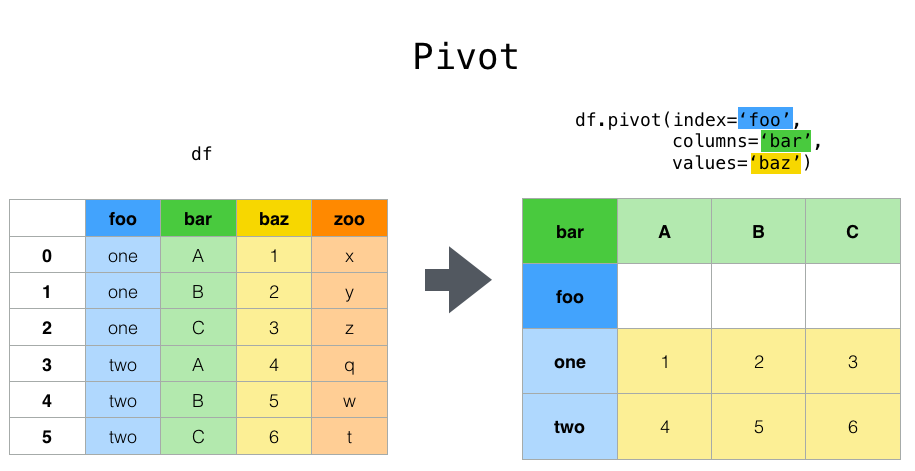
\includegraphics[width=0.85\textwidth]{figures/pandas/reshaping_pivot.png}
\caption{
Example \pandas \texttt{pivot} operation, from the package \href{http://pandas.pydata.org/pandas-docs/stable/user_guide/reshaping.html}{documentation}.
}
\label{fig:pandas:pivot}
\end{figure}

\subsubsection{pivot\_table}
\label{pandas:pivoting:pivot_table}

\noindent \href{https://pandas.pydata.org/pandas-docs/stable/reference/api/pandas.pivot_table.html}{\texttt{pivot\_table} documentation}.

\begin{lstlisting}[language=Python]
pandas.pivot_table(data, values=None, index=None, columns=None, aggfunc='mean', fill_value=None, margins=False, dropna=True, margins_name='All')
\end{lstlisting}

\begin{figure}[H]
\centering
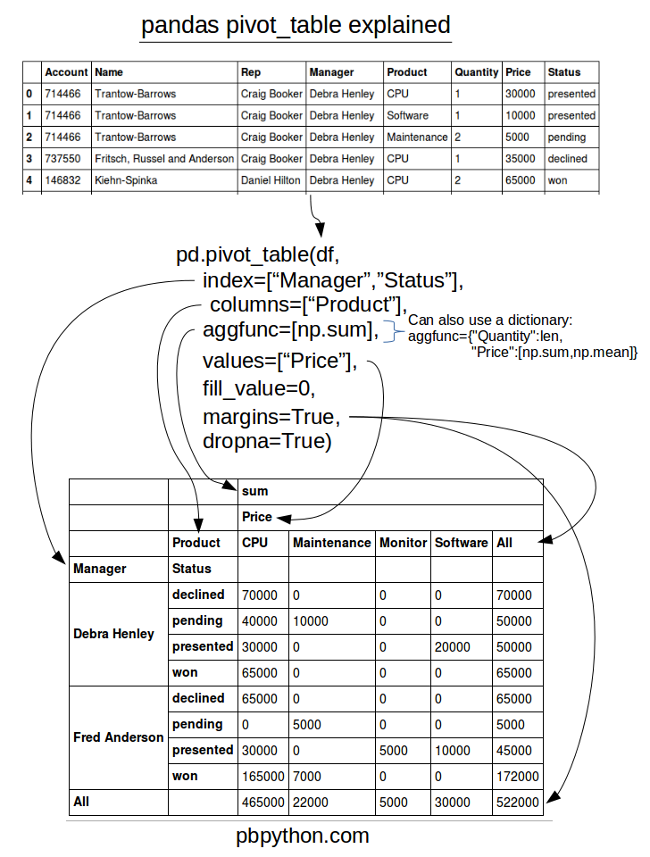
\includegraphics[width=0.95\textwidth]{figures/pandas/pivot-table-datasheet.png}
\caption{
Example \pandas \texttt{pivot\_table} operation, by \href{http://pbpython.com/pandas-pivot-table-explained.html}{Chris Moffitt}.
}
\label{fig:pandas:pivot_table}
\end{figure}
}
%%%%%%%%%%%%%%%%%%%%%%%%%%%%%%%%%%%%%%%%%%%%%%%%%%%%%%%%
%%%%%%%%%%%%%%%%%%%%%%%%%%%%%%%%%%%%%%%%%%%%%%%%%%%%%%%%
\chapter{\sql}
\label{sql}

%%%%%%%%%%%%%%%%%%%%%%%%%%%%%%%%%%%%%%%%%%%%%%%%%%%%%%%%
%%%%%%%%%%%%%%%%%%%%%%%%%%%%%%%%%%%%%%%%%%%%%%%%%%%%%%%%
\section{Basic Commands}
\label{sql:basic}
% TODO

}
%%%%%%%%%%%%%%%%%%%%%%%%%%%%%%%%%%%%%%%%%%%%%%%%%%%%%%%%
%%%%%%%%%%%%%%%%%%%%%%%%%%%%%%%%%%%%%%%%%%%%%%%%%%%%%%%%
\chapter{Additional Methods}
\label{additional}

While interesting, the methods covered in this appendix are less likely
to be relevant during the interview process.

%%%%%%%%%%%%%%%%%%%%%%%%%%%%%%%%%%%%%%%%%%%%%%%%%%%%%%%%
%%%%%%%%%%%%%%%%%%%%%%%%%%%%%%%%%%%%%%%%%%%%%%%%%%%%%%%%
\section{Statistics}
\label{additional:stats}

%%%%%%%%%%%%%%%%%%%%%%%%%%%%%%%%%%%%%%%%%%%%%%%%%%%%%%%%
\subsection{Analysis of Variance (ANOVA)}
\label{additional:stats:ANOVA}
% TODO

%%%%%%%%%%%%%%%%%%%%%%%%%%%%%%%%%%%%%%%%%%%%%%%%%%%%%%%%
\subsection{Time Series Analysis}
\label{additional:stats:time_series_ana}
% TODO

%%%%%%%%%%%%%%%%%%%%%%%%%%%%%%%%%%%%%%%%%%%%%%%%%%%%%%%%
%%%%%%%%%%%%%%%%%%%%%%%%%%%%%%%%%%%%%%%%%%%%%%%%%%%%%%%%
\section{Regression}
\label{additional:Regression}

%%%%%%%%%%%%%%%%%%%%%%%%%%%%%%%%%%%%%%%%%%%%%%%%%%%%%%%%
\subsection{Principal Component Regression (PCR)}
\label{additional:Regression:PCR}
% TODO

%%%%%%%%%%%%%%%%%%%%%%%%%%%%%%%%%%%%%%%%%%%%%%%%%%%%%%%%
\subsection{Generalized Linear Models (GLM)}
\label{additional:Regression:GLM}
% TODO

%%%%%%%%%%%%%%%%%%%%%%%%%%%%%%%%%%%%%%%%%%%%%%%%%%%%%%%%
\subsection{Poisson Regression}
\label{additional:Regression:poisson}
% TODO

%%%%%%%%%%%%%%%%%%%%%%%%%%%%%%%%%%%%%%%%%%%%%%%%%%%%%%%%
%%%%%%%%%%%%%%%%%%%%%%%%%%%%%%%%%%%%%%%%%%%%%%%%%%%%%%%%
\section{Unsupervised Learning}
\label{additional:unsupervised}

%%%%%%%%%%%%%%%%%%%%%%%%%%%%%%%%%%%%%%%%%%%%%%%%%%%%%%%%
\subsection{Gaussian Mixture Model (GMM)}
\label{additional:unsupervised:GMM}
% TODO

%%%%%%%%%%%%%%%%%%%%%%%%%%%%%%%%%%%%%%%%%%%%%%%%%%%%%%%%
\subsection{\texorpdfstring{$\epsilon$}{epsilon}-Means}
\label{additional:unsupervised:epsilonMean}
% TODO

%%%%%%%%%%%%%%%%%%%%%%%%%%%%%%%%%%%%%%%%%%%%%%%%%%%%%%%%
\subsection{Louvain Method}
\label{additional:unsupervised:louvain}
% TODO

%%%%%%%%%%%%%%%%%%%%%%%%%%%%%%%%%%%%%%%%%%%%%%%%%%%%%%%%
%%%%%%%%%%%%%%%%%%%%%%%%%%%%%%%%%%%%%%%%%%%%%%%%%%%%%%%%
\section{Supervised Learning}
\label{additional:supervised}

%%%%%%%%%%%%%%%%%%%%%%%%%%%%%%%%%%%%%%%%%%%%%%%%%%%%%%%%
\subsection{Adversarial Networks} % TODO (AN?)
\label{additional:supervised:AN}
% TODO

%%%%%%%%%%%%%%%%%%%%%%%%%%%%%%%%%%%%%%%%%%%%%%%%%%%%%%%%
\subsection{Variational Autoencoders (VAE)}
\label{additional:supervised:VAE}
% TODO

\subsection{Learning Vector Quantization (LVQ)}
\label{additional:supervised:kNN:LVQ}
% TODO

%%%%%%%%%%%%%%%%%%%%%%%%%%%%%%%%%%%%%%%%%%%%%%%%%%%%%%%%
%%%%%%%%%%%%%%%%%%%%%%%%%%%%%%%%%%%%%%%%%%%%%%%%%%%%%%%%
\section{Miscellaneous}
\label{additional:misc}

%%%%%%%%%%%%%%%%%%%%%%%%%%%%%%%%%%%%%%%%%%%%%%%%%%%%%%%%
\subsection{Factor Analysis}
\label{additional:misc:factor_ana}
% TODO

}
%%%%%%%%%%%%%%%%%%%%%%%%%%%%%%%%%%%%%%%%%%%%%%%%%%%%%%%%
%%%%%%%%%%%%%%%%%%%%%%%%%%%%%%%%%%%%%%%%%%%%%%%%%%%%%%%%
%%%%%%%%%%%%%%%%%%%%%%%%%%%%%%%%%%%%%%%%%%%%%%%%%%%%%%%%
\chapter{Concepts for Finance}
\label{finance}

%%%%%%%%%%%%%%%%%%%%%%%%%%%%%%%%%%%%%%%%%%%%%%%%%%%%%%%%
%%%%%%%%%%%%%%%%%%%%%%%%%%%%%%%%%%%%%%%%%%%%%%%%%%%%%%%%
\section{Stochastic Processes}
\label{finance:sp}
% TODO

%%%%%%%%%%%%%%%%%%%%%%%%%%%%%%%%%%%%%%%%%%%%%%%%%%%%%%%%
%%%%%%%%%%%%%%%%%%%%%%%%%%%%%%%%%%%%%%%%%%%%%%%%%%%%%%%%
\section{Martingale}
\label{finance:martingale}
% TODO

%%%%%%%%%%%%%%%%%%%%%%%%%%%%%%%%%%%%%%%%%%%%%%%%%%%%%%%%
%%%%%%%%%%%%%%%%%%%%%%%%%%%%%%%%%%%%%%%%%%%%%%%%%%%%%%%%
\section{Wiener Processes}
\label{finance:wiener}
% TODO

%%%%%%%%%%%%%%%%%%%%%%%%%%%%%%%%%%%%%%%%%%%%%%%%%%%%%%%%
%%%%%%%%%%%%%%%%%%%%%%%%%%%%%%%%%%%%%%%%%%%%%%%%%%%%%%%%
\section{Brownian Motion}
\label{finance:brownian}
% TODO

%%%%%%%%%%%%%%%%%%%%%%%%%%%%%%%%%%%%%%%%%%%%%%%%%%%%%%%%
%%%%%%%%%%%%%%%%%%%%%%%%%%%%%%%%%%%%%%%%%%%%%%%%%%%%%%%%
\section{Random Walks}
\label{finance:rand_walk}
% TODO

%%%%%%%%%%%%%%%%%%%%%%%%%%%%%%%%%%%%%%%%%%%%%%%%%%%%%%%%
%%%%%%%%%%%%%%%%%%%%%%%%%%%%%%%%%%%%%%%%%%%%%%%%%%%%%%%%
\section{It\^o's Lemma}
\label{finance:ito_lemma}
% TODO

%%%%%%%%%%%%%%%%%%%%%%%%%%%%%%%%%%%%%%%%%%%%%%%%%%%%%%%%
%%%%%%%%%%%%%%%%%%%%%%%%%%%%%%%%%%%%%%%%%%%%%%%%%%%%%%%%
\section{Black-Scholes Model}
\label{finance:black_scholes}
% TODO

}

%-----------------------------------------------------------------------------%
% BIBLIOGRAPHY -- Change the style to match your discipline's standards.
%-----------------------------------------------------------------------------%
\bibliographystyle{./bib/atlasBibStyleWithTitle}
\cleardoublepage
\normalbaselines %Fixes spacing of bibliography
% \addcontentsline{toc}{chapter}{Bibliography} % not needed on my system
\bibliography{./bib/bib}
%-----------------------------------------------------------------------------%

%-----------------------------------------------------------------------------
\end{document}
